% id: 78-04
% book: 100발100중 3-2 중간 · 01 3-2 중간(삼각비·삼각비의 활용·원과 직선·원주각·부록)
% section: 기출 Best
% figure: crop:fig-78-04.png
% answer: ④
% answer_source: 답지(빠른정답)
% variant_level: 0 (원본 전사)
% 이 파일은 build.mjs 가 items.json 에서 만든다. 고칠 때는 items.json 을 고친다.
\smash{\raisebox{1.5mm}{\dmkichul{100발100중 3-2 중간 78쪽 04번}}}
\noindent\begin{minipage}[t]{0.58\linewidth}\vspace{0pt}\raggedright 그림에서 $\overrightarrow{\pt{PA}}$, $\overrightarrow{\pt{PB}}$는 원~$\pt{O}$의 접선이고 두 점~$\pt{A}$, $\pt{B}$는 접점이다. $\angle\pt{APB}=50^\circ$일 때, $\angle x$의 크기는?\end{minipage}\hfill\begin{minipage}[t]{0.4\linewidth}\vspace{0pt}\centering 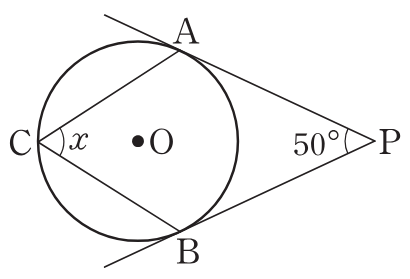
\includegraphics[width=98.2pt]{figures/fig-78-04.png}\end{minipage}\par
\begin{choices32}{$50^\circ$}{$55^\circ$}{$60^\circ$}{$65^\circ$}{$70^\circ$}\end{choices32}
